
\documentclass{beamer}

% official, as per http://www.uvm.edu/~mmetivie/?Page=rules_logo.html
% Green: R:0 G:104 B:71
% white: R:255 G:250 B:250 

\definecolor{green}{RGB}{0,104,71}
\definecolor{white}{RGB}{255,250,250}

\usepackage{gensymb}

\usepackage{graphicx}
\graphicspath{{./img/}}

\mode<presentation>
{
  \usetheme{default}
  \setbeamertemplate{navigation symbols}{}
  \setbeamercolor{titlelike}{fg=white,bg=green}
  \useinnertheme[shadow=true]{rounded}
  \setbeamercolor{item projected}{fg=green,bg=green!20}
  \setbeamertemplate{blocks}[rounded][shadow=true]
}

\title[]{\textit{Aphaenogaster} sampling}

\author{John Stanton-Geddes}

\institute{Department of Biology \\ University of Vermont}

\setlength{\parskip}{14.0pt plus 8.0pt minus 3.0pt}

\begin{document}

\begin{frame}
  \titlepage
\end{frame}


\begin{frame}{Latitudinal variation in gene expression}
	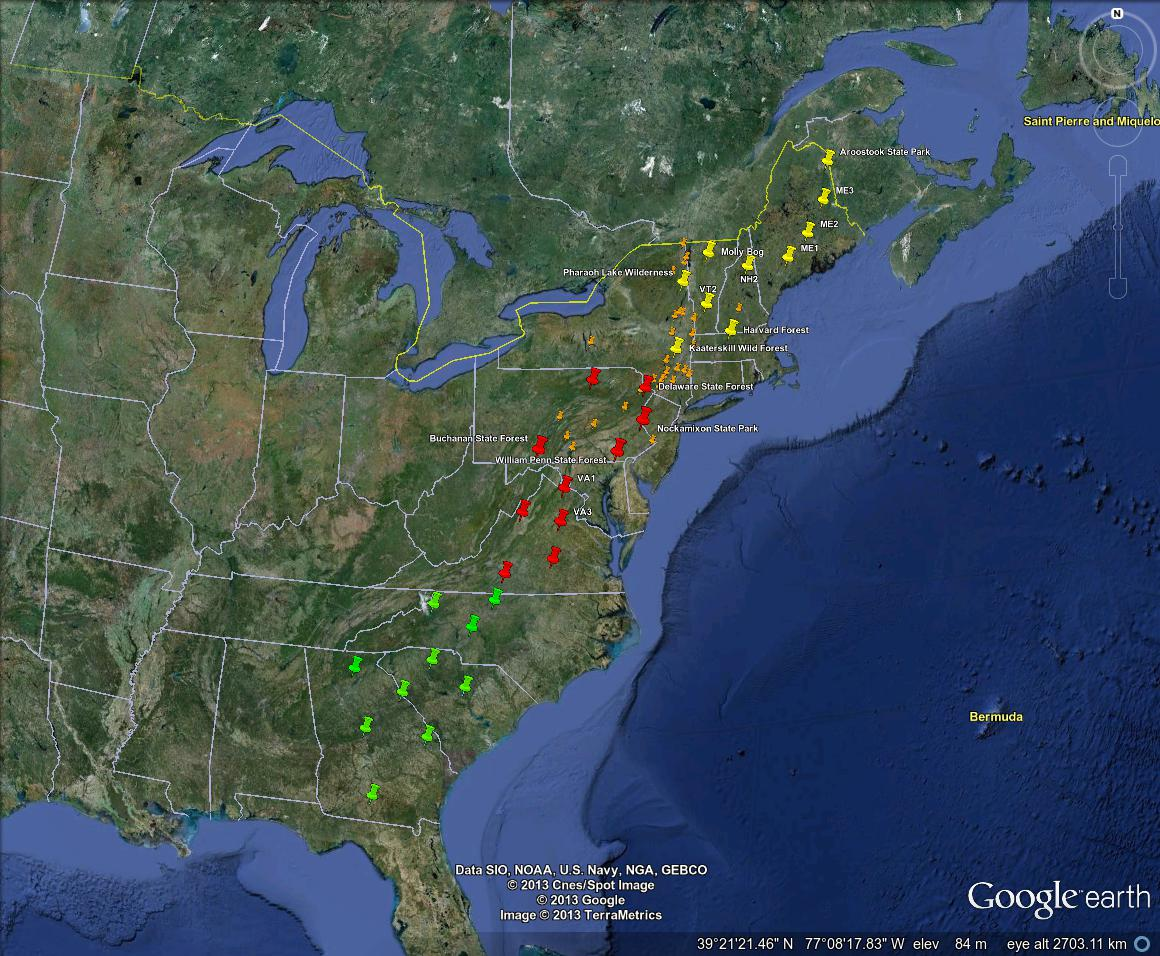
\includegraphics[width=\textwidth, height=\textheight, keepaspectratio]{Aphaenogaster2013_sampling_locations_20130313.jpg}
\end{frame}


\begin{frame}{Latitudinal variation in gene expression}
	\begin{block}{Goals}
		\begin{enumerate}
			\item Identify genes underlying differences among populations in thermal tolerance
			\item Evaluate the extent to which selection has acted on climate-related genes
		\end{enumerate}
	\end{block}
\end{frame}


\begin{frame}{Latitudinal variation in gene expression}
	\begin{center}
		\Large{Ovation 3' Digital Gene Expression (DGE) Tags}
		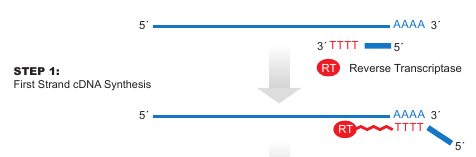
\includegraphics[width=8cm]{ovation_DGE.png}\\
	\end{center}
\end{frame}


\begin{frame}{Latitudinal variation in gene expression}
	\begin{center}
		\large{Common gardens for gene expression}
		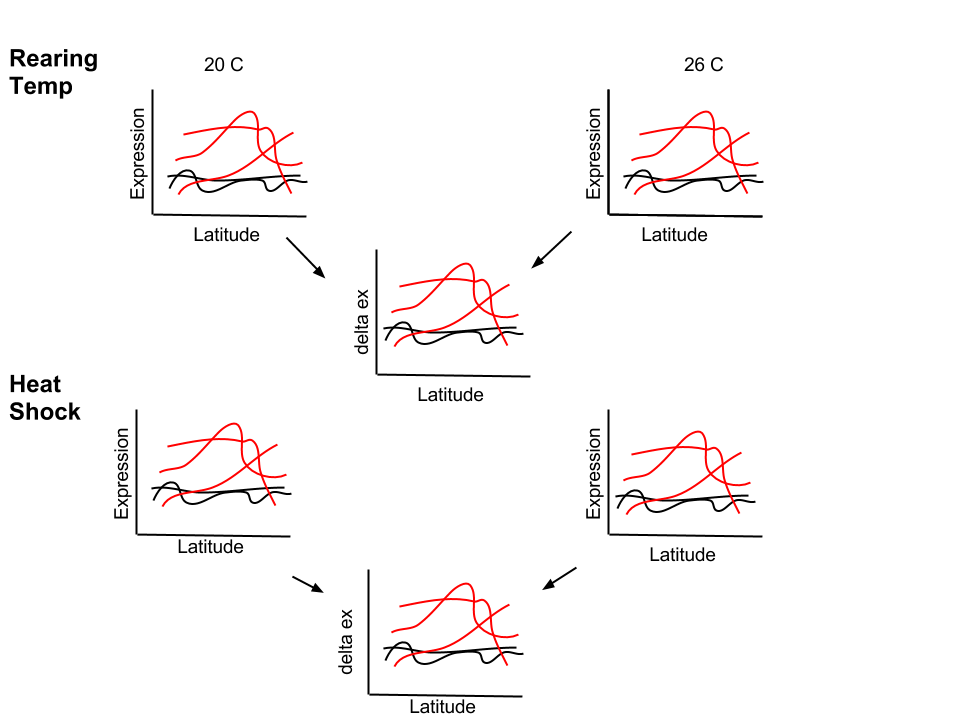
\includegraphics[width=8cm]{Latitudinal_gene_expression.png}\\
	\end{center}
\end{frame}


\begin{frame}{Latitudinal variation in gene expression}
	\begin{block}{Challenges}
		\begin{enumerate}
			\item A. picea and A. rudis
			\item 
		\end{enumerate}
	\end{block}
\end{frame}


\begin{frame}{Population genomics of \textit{Aphaenogaster}}
	\begin{columns}
		\begin{column}{5cm}

			SNPs in 3' tail of gene expression tags
			\vspace{1cm}

			\includegraphics<1>[width=5cm]{ovation_DGE.png}\\
		\end{column}
		\begin{column}{5cm}
			\begin{center}
				\begin{itemize}
					\item Do genes with significant changes in expression among sites have reduced molecular diversity? different haplotypes?
					\item How are populations structured?
					\item What is the extent of gene flow? Male vs female dispersal?
				\end{itemize}
			\end{center}
		\end{column}
	\end{columns}
\end{frame}


\end{document}

